%-------------------------------------------------------------------------
% Informe Tarea 2: Demosaicking neuronal y basado en fisica
%-------------------------------------------------------------------------
\documentclass[a4paper,11pt]{article}

\usepackage[a4paper,margin=2.5cm]{geometry}
\usepackage[T1]{fontenc}
\usepackage[utf8]{inputenc}
\usepackage[spanish]{babel}
\usepackage{amsmath,amssymb}
\usepackage{booktabs}
\usepackage{graphicx}
\usepackage{hyperref}
\usepackage{xcolor}
\usepackage{listings}

\hypersetup{colorlinks=true,linkcolor=blue,urlcolor=blue,citecolor=blue}
\setlength{\parindent}{0pt}
\setlength{\parskip}{0.55em}

\lstset{
    language=Python,
    basicstyle=\small\ttfamily,
    breaklines=true,
    frame=single,
    showstringspaces=false,
    columns=fullflexible
}

\title{
    
\includegraphics[width=5cm]{Fig/usm.png}\\[0.8cm]
    \large Universidad Técnica Federico Santa María\\
    \large Departamento de Informática\\[0.5cm]
    \LARGE\textbf{Informe Tarea 2}\\[0.2cm]
    \Large Demosaicking RGB mediante representaciones implícitas y redes convolucionales
}

\author{Francisco Alfaro Medina}
\date{Septiembre de 2026}

\begin{document}

\maketitle

\begin{abstract}
En este trabajo se reconstruye una imagen RGB a partir de una medición mosaico Bayer proveniente de un archivo digital negativo (DNG). Se comparan una interpolación bilineal, el demosaicking de OpenCV, una representación neuronal implícita tipo INR-SIREN y una red neuronal convolucional. La CNN se entrena con parches de imágenes Kodak y se evalúa sobre imágenes no vistas. Además, se implementa una arquitectura encoder--decoder inspirada en la Figura 3 del enunciado y una variante con mayor capacidad. Finalmente, los métodos se aplican a una captura DNG real, incorporando revelado con \texttt{rawpy}, corrección de color y gamma sRGB. En la prueba controlada la INR-SIREN obtuvo el mejor resultado, mientras que en Kodak la interpolación bilineal superó a la CNN entrenada. La CNN mejorada redujo el error respecto de la arquitectura base, aunque no alcanzó todavía el desempeño de la línea base clásica.
\end{abstract}

\section{Introducción}

Un sensor de imagen con filtro Bayer registra una sola intensidad por posición espacial. El patrón de filtros asigna cada píxel a uno de los canales rojo, verde o azul, por lo que la medición contiene información incompleta para formar una imagen RGB. El objetivo del demosaicking es estimar los dos canales faltantes en cada posición y reconstruir una imagen de tres canales.

El enunciado solicita implementar métodos neuronales para recuperar RGB desde datos RAW/DNG, comparar los resultados con el procesamiento de la cámara y con algoritmos clásicos, y estudiar el efecto de modificar la arquitectura o la estrategia de entrenamiento. En particular, se consideran una representación implícita y una CNN basada en la arquitectura de la Figura 3.

\section{Datos y diseño experimental}

Se utilizó el archivo \texttt{demo.dng}, descargado desde un repositorio público, junto con \texttt{demo.jpg} como referencia visual procesada por la cámara. Esta elección corresponde a la alternativa indicada en el enunciado para el caso en que no se disponga de una captura RAW propia de un teléfono. El DNG tiene una medición visible de tamaño $3060\times4080$ y el JPG tiene tamaño $4080\times3060\times3$.

También se utilizó el conjunto Kodak, compuesto por 24 imágenes RGB. Se reservaron 20 imágenes para entrenamiento y 4 imágenes completas para prueba. Cada imagen se dividió en parches de $64\times64$, obteniéndose 1920 parches de entrenamiento y 384 parches de prueba. Las imágenes de prueba no fueron utilizadas durante el entrenamiento.

Al leer el DNG con \texttt{rawpy}, se obtuvo el patrón CFA:

\[
\begin{bmatrix}
G & R\\
B & G
\end{bmatrix},
\qquad \text{patrón } GRBG.
\]

Los niveles negro reportados fueron $[63,63,63,63]$ y el nivel blanco fue 1023. La medición se normalizó después de descontar el nivel negro y se acotó al intervalo $[0,1]$.

\begin{figure}[!ht]
\centering
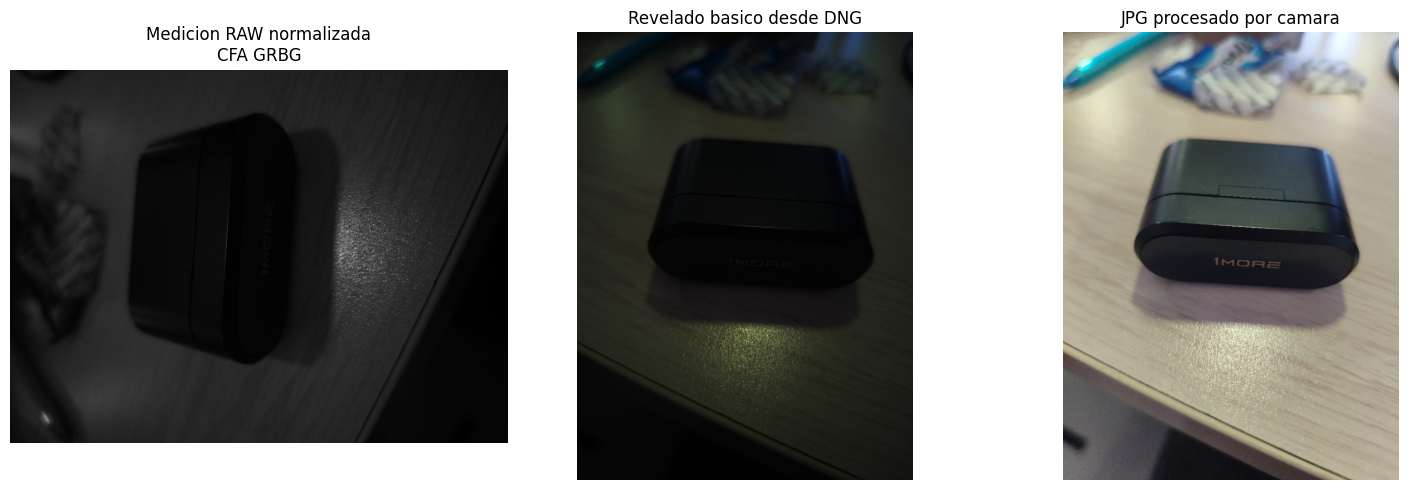
\includegraphics[width=0.98\linewidth]{Fig/dng_rawpy_jpg.png}
\caption{Medición RAW normalizada, revelado básico mediante \texttt{rawpy} y JPG procesado por la cámara.}
\label{fig:dng_rawpy_jpg}
\end{figure}

\section{Métodos}

\subsection{Modelo de mosaico Bayer}

Sea $I\in\mathbb{R}^{H\times W\times3}$ una imagen RGB y sean $M_R$, $M_G$ y $M_B$ las máscaras binarias del patrón Bayer. La medición mosaico se construye como

\[
Y=M_R\odot I_R+M_G\odot I_G+M_B\odot I_B.
\]

Para la CNN, la entrada se representa como cuatro canales:

\[
X=[Y,M_R,M_G,M_B],
\]

mientras que la salida esperada corresponde a la imagen RGB completa.

\subsection{Interpolación bilineal y OpenCV}

La interpolación bilineal reconstruye cada canal por separado utilizando únicamente las muestras conocidas y filtros locales $3\times3$. Para rojo y azul se empleó

\[
H_{R,B}=\begin{bmatrix}1&2&1\\2&4&2\\1&2&1\end{bmatrix},
\]

y para verde,

\[
H_G=\begin{bmatrix}0&1&0\\1&4&1\\0&1&0\end{bmatrix}.
\]

Como segunda línea base se utilizó \texttt{cv2.cvtColor} con la conversión Bayer correspondiente al patrón \texttt{GRBG}. La salida BGR de OpenCV se invirtió a RGB para mantener la convención utilizada por el resto del notebook.

\subsection{Representación neuronal implícita}

La INR-SIREN representa la imagen como una función neuronal continua de las coordenadas espaciales $(x,y)$. La red recibe las coordenadas normalizadas y produce tres intensidades RGB. Sus parámetros se optimizan directamente sobre el mosaico observado, utilizando una pérdida de consistencia con las muestras Bayer conocidas. Este procedimiento se realiza para la imagen específica, por lo que puede obtener un ajuste muy preciso, pero requiere volver a entrenar la representación para cada captura.

\subsection{CNN inspirada en la Figura 3}

La CNN implementada utiliza una arquitectura encoder--decoder. El encoder reduce la resolución mediante convoluciones con stride y capas de pooling. En el cuello de botella se utilizan bloques residuales. El decoder recupera la resolución mediante convoluciones transpuestas y suma características de distintas escalas mediante conexiones tipo \texttt{add}.

Para un parche de entrada de $64\times64$, la representación se reduce hasta $4\times4$ y luego se reconstruye hasta $64\times64$. La CNN base utiliza 16 canales ocultos y 4 bloques residuales. La salida se limita al intervalo $[0,1]$ mediante una función sigmoide.

La función de entrenamiento combina una pérdida RGB supervisada con una pérdida de consistencia física:

\[
\mathcal{L}=\mathcal{L}_{RGB}+\lambda\mathcal{L}_{\mathrm{fisica}},
\]

donde la segunda componente penaliza que la reconstrucción no reproduzca la medición Bayer observada. Se utilizaron seis épocas y $\lambda=0.1$ en la CNN base.

\subsection{Variante mejorada}

Para estudiar el efecto de aumentar la capacidad, se entrenó una variante con 32 canales ocultos y 6 bloques residuales. También se entrenó una versión de la misma arquitectura con $\lambda=0$, eliminando la pérdida de consistencia física. Las tres variantes utilizaron las mismas imágenes, parches y número de épocas.

\subsection{Revelado y corrección de color del DNG}

El DNG no es una imagen RGB lista para visualizar. Por esta razón, el revelado de referencia se realizó con \texttt{rawpy} usando el balance de blancos de la cámara, salida de 16 bits, espacio sRGB, gamma $(1,1)$ y demosaicking AHD. Sobre las reconstrucciones obtenidas por los diferentes métodos se aplicó una matriz de corrección de color:

\[
C=\begin{bmatrix}
1.50&-0.30&-0.20\\
-0.20&1.30&-0.10\\
-0.10&-0.20&1.30
\end{bmatrix}.
\]

Si $\hat I$ es una reconstrucción RGB lineal normalizada, la corrección se calcula como

\[
\hat I_{cc}(i,j)=C\hat I(i,j),
\]

seguida de una conversión de RGB lineal a sRGB para visualización. La misma matriz y la misma gamma se aplicaron a las salidas del DNG de la interpolación bilineal, OpenCV, CNN e INR-SIREN.

\section{Métricas}

Se utilizaron MSE, PSNR y SSIM. El error cuadrático medio se define como

\[
\operatorname{MSE}(I,\hat I)=\frac{1}{3HW}
\sum_{i,j,c}(I_c(i,j)-\hat I_c(i,j))^2.
\]

El PSNR se calculó con rango dinámico 1:

\[
\operatorname{PSNR}=10\log_{10}\left(\frac{1}{\operatorname{MSE}}\right).
\]

SSIM se utilizó como medida complementaria de similitud estructural. En todas las métricas, un MSE menor y valores mayores de PSNR y SSIM indican una mejor reconstrucción.

\section{Resultados}

\subsection{Prueba controlada con \texttt{demo.jpg}}

Se generó un mosaico Bayer sintético a partir de \texttt{demo.jpg}, por lo que en esta prueba se conoce la imagen RGB original antes del mosaico.

\begin{table}[!ht]
\centering
\caption{Resultados de la prueba controlada con \texttt{demo.jpg}.}
\label{tab:controlado}
\begin{tabular}{lrrr}
\toprule
Método & MSE & PSNR [dB] & SSIM\\
\midrule
Interpolación bilineal & 0.0002 & 36.0545 & 0.9690\\
OpenCV & 0.0084 & 20.7544 & 0.9053\\
INR-SIREN & 0.0001 & 41.0670 & 0.9791\\
\bottomrule
\end{tabular}
\end{table}

La INR-SIREN obtuvo el mejor resultado en las tres métricas. Esta ventaja es consistente con el hecho de que la INR se optimiza específicamente para la captura evaluada. La interpolación bilineal también obtuvo un resultado alto, mientras que OpenCV presentó un error considerablemente mayor en esta implementación.

\begin{figure}[!ht]
\centering
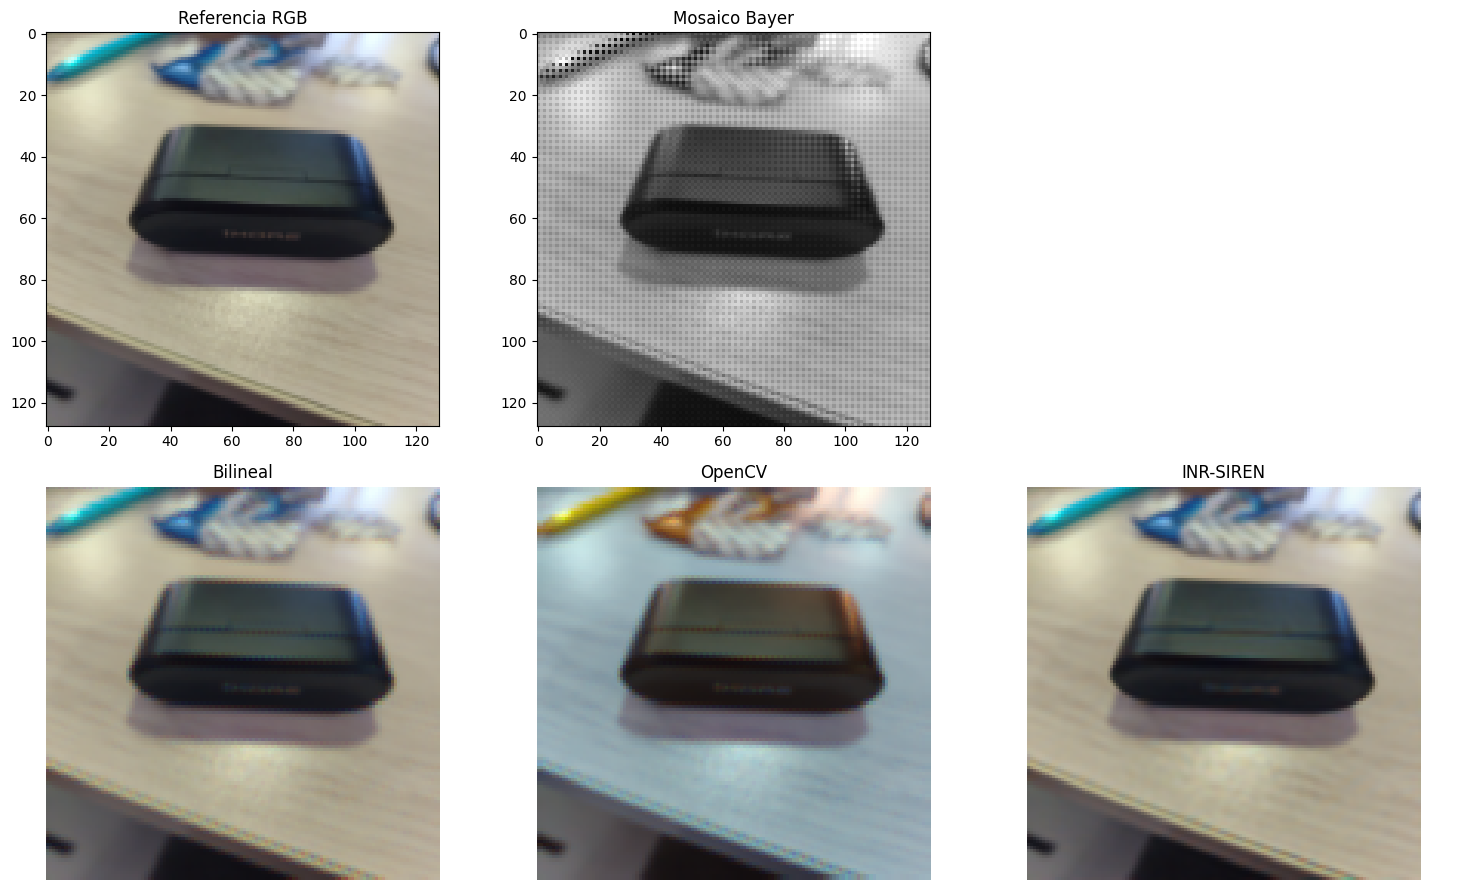
\includegraphics[width=0.98\linewidth]{Fig/comparacion_controlada.png}
\caption{Comparación visual en la prueba controlada: referencia RGB, mosaico Bayer y reconstrucciones.}
\label{fig:comparacion_controlada}
\end{figure}

\begin{figure}[!ht]
\centering
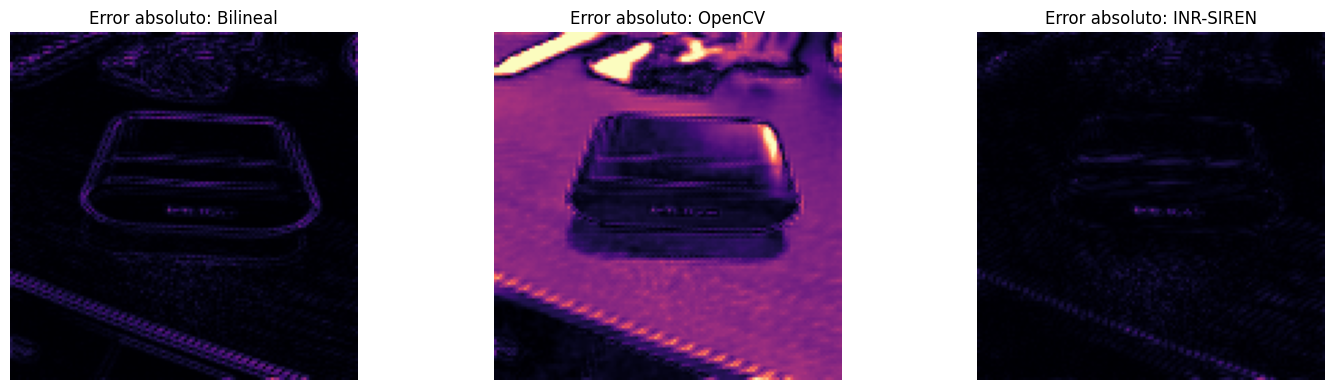
\includegraphics[width=0.98\linewidth]{Fig/errores_controlado.png}
\caption{Mapas de error absoluto amplificado para la prueba controlada.}
\label{fig:errores_controlado}
\end{figure}

\subsection{Generalización sobre Kodak}

\begin{table}[!ht]
\centering
\caption{Resultados promedio sobre parches de prueba Kodak.}
\label{tab:kodak}
\begin{tabular}{lrrr}
\toprule
Método & MSE & PSNR [dB] & SSIM\\
\midrule
Interpolación bilineal & 0.0013 & 33.4489 & 0.9060\\
OpenCV & 0.0261 & 19.1799 & 0.7996\\
CNN multi-imagen & 0.0058 & 23.8272 & 0.7329\\
\bottomrule
\end{tabular}
\end{table}

En Kodak, la interpolación bilineal superó a la CNN base en las tres métricas. La CNN obtuvo un MSE aproximadamente 4.4 veces mayor que la bilineal y una diferencia de 9.62 dB en PSNR. Por lo tanto, la red aprendió a realizar una reconstrucción, pero su generalización no fue suficiente para superar a la línea base clásica con el entrenamiento utilizado.

\subsection{Variantes de la CNN}

\begin{table}[!ht]
\centering
\caption{Comparación de variantes de arquitectura y pérdida.}
\label{tab:variantes}
\begin{tabular}{lrrrrr}
\toprule
Método & Canales & Bloques & $\lambda$ & MSE prueba & Tiempo [s]\\
\midrule
CNN Figura 3 & 16 & 4 & 0.1 & 0.0050 & 4.9475\\
CNN mejorada & 32 & 6 & 0.1 & 0.0033 & 5.4917\\
CNN mejorada sin física & 32 & 6 & 0.0 & 0.0034 & 6.0720\\
\bottomrule
\end{tabular}
\end{table}

La CNN mejorada redujo el MSE de 0.0050 a 0.0033, lo que corresponde a una disminución aproximada de 34\%. La eliminación de la pérdida física aumentó ligeramente el error a 0.0034. En esta corrida, el aumento de canales y bloques tuvo un efecto más importante que la pérdida física, aunque la consistencia física produjo una mejora pequeña frente a la arquitectura equivalente sin ella.

\begin{figure}[!ht]
\centering
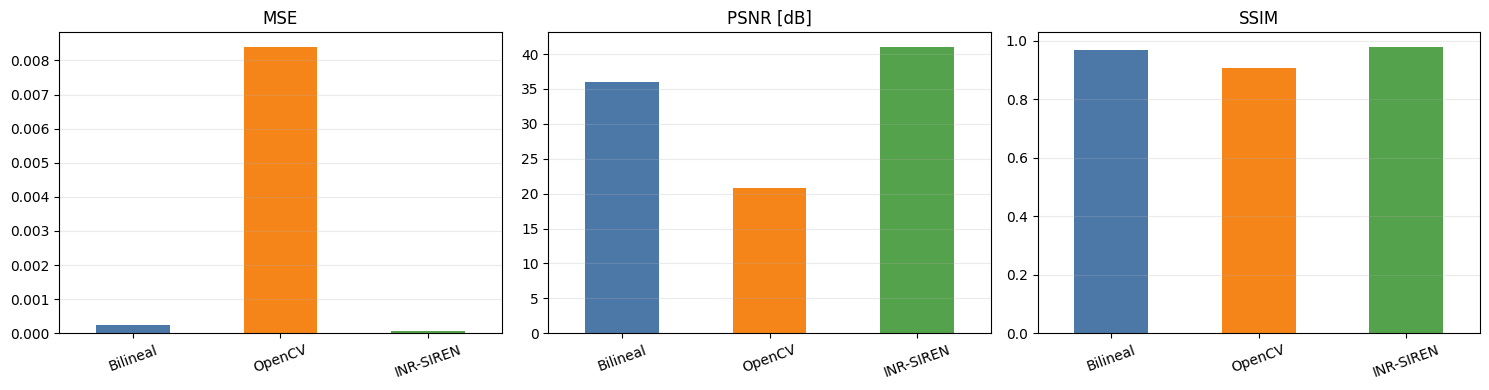
\includegraphics[width=0.98\linewidth]{Fig/metricas_controlado.png}
\caption{MSE, PSNR y SSIM obtenidos en la prueba controlada.}
\label{fig:metricas_controlado}
\end{figure}

\subsection{Visualización de la captura DNG real}

La Figura~\ref{fig:dng_metodos_color} muestra el recorte central de la captura real después de aplicar la corrección de color y la conversión a sRGB. La comparación permite observar diferencias de color, ruido, nitidez y artefactos entre los métodos. En particular, la salida de la CNN presenta una cuadrícula visible en este recorte, lo que sugiere que el modelo todavía tiene dificultades al transferir el conocimiento aprendido en Kodak a una medición real de cámara.

\begin{figure}[!ht]
\centering
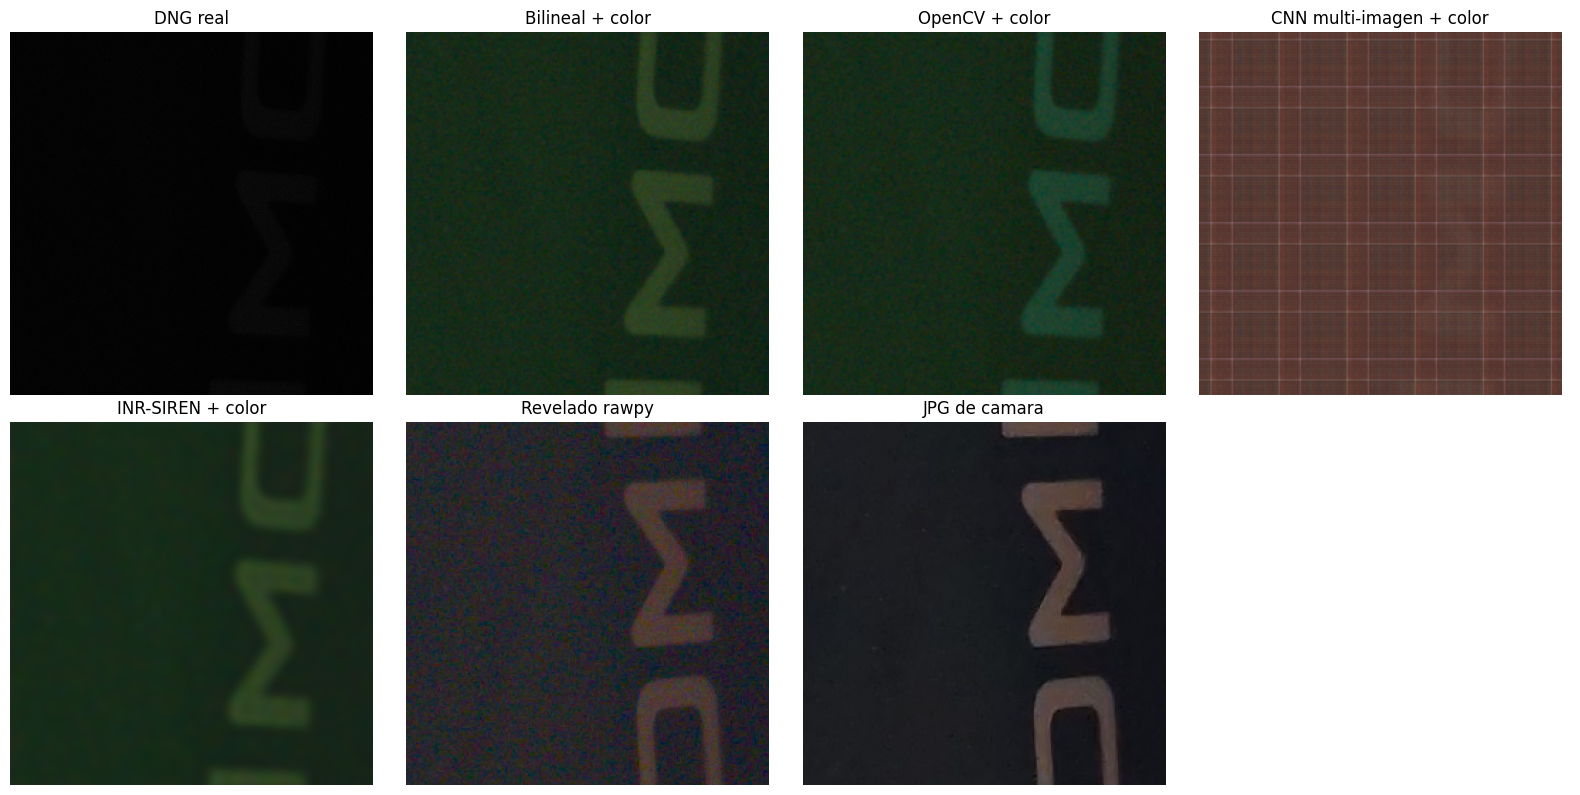
\includegraphics[width=0.98\linewidth]{Fig/dng_metodos_color.png}
\caption{Reconstrucciones sobre el DNG real después de la corrección de color, comparadas con el revelado de \texttt{rawpy} y el JPG de la cámara.}
\label{fig:dng_metodos_color}
\end{figure}

\section{Análisis}

La pérdida de entrenamiento de la CNN principal disminuyó de 0.038695 a 0.006798 durante seis épocas. Esto indica que la red pudo aprender la relación entre el mosaico Bayer y la imagen RGB objetivo. Sin embargo, la diferencia entre el desempeño de entrenamiento y el resultado de prueba muestra que todavía existen dificultades de generalización hacia imágenes no vistas. El conjunto de entrenamiento es pequeño y las imágenes utilizadas para formar los parches tienen una distribución limitada.

La INR-SIREN fue superior en la prueba controlada, pero la comparación no es completamente equivalente a la de la CNN: la INR se ajusta directamente a la imagen de evaluación, mientras que la CNN busca aprender una regla general a partir de varias imágenes. En consecuencia, la INR funciona como un ajuste específico de captura y la CNN como un modelo reutilizable. La alta calidad de la INR no implica necesariamente una mejor capacidad de generalización.

El resultado de OpenCV fue peor que el de la interpolación bilineal, tanto en la prueba controlada como en Kodak. Dado que OpenCV normalmente constituye una línea base competitiva, esta diferencia debe interpretarse como un resultado de la implementación concreta y no como una conclusión general sobre OpenCV. Es necesario verificar cuidadosamente la correspondencia entre el patrón \texttt{GRBG}, las convenciones BGR/RGB y la escala de los datos de entrada. Una inversión de canales o una codificación Bayer incorrecta puede aumentar considerablemente el error.

Para la captura real, el JPG corresponde al resultado del pipeline incorporado de la cámara, mientras que \texttt{rawpy} proporciona un revelado independiente. Ambos incluyen decisiones de balance de blancos, color y tono que no están presentes en el mosaico RAW. Por ello, la comparación del DNG se realizó de forma cualitativa después de aplicar corrección de color y gamma sRGB, y no se utilizaron métricas contra el JPG como si este fuera una verdad de terreno lineal.

\section{Conclusiones}

Se implementó un flujo completo de demosaicking desde una captura DNG real y desde mosaicos sintéticos. El trabajo incluyó una línea base bilineal, OpenCV, una representación neuronal implícita y una CNN encoder--decoder inspirada en la arquitectura de la Figura 3. También se entrenó una variante mejorada con más canales y bloques residuales.

En la prueba controlada, la INR-SIREN obtuvo el mejor desempeño, con PSNR de 41.0670 dB y SSIM de 0.9791. Este resultado se explica por su optimización específica para la captura. En las imágenes Kodak no vistas, la interpolación bilineal fue el método más preciso de los evaluados, con PSNR de 33.4489 dB y SSIM de 0.9060. La CNN base alcanzó PSNR de 23.8272 dB y SSIM de 0.7329, por lo que aún requiere más entrenamiento, datos o ajustes para superar la línea base.

La modificación de la arquitectura fue positiva: la CNN mejorada redujo el MSE de prueba en aproximadamente 34\% respecto de la CNN Figura 3. La pérdida de consistencia física aportó una mejora marginal en esta corrida. Esto muestra que aumentar la capacidad de representación ayudó más que modificar solamente el término físico de la función de pérdida.

Finalmente, los resultados sobre el DNG real fueron revelados mediante \texttt{rawpy} y las reconstrucciones fueron transformadas a un espacio de color visualizable mediante una matriz de corrección de color y gamma sRGB. La comparación con el JPG del teléfono es útil para inspección cualitativa, pero no debe interpretarse como una métrica objetiva porque el JPG ya incluye procesamiento interno de la cámara.

\section*{Archivos entregados}

El informe se acompaña de los archivos \texttt{homework2.ipynb} y \texttt{Demosaicked-colorCorrection.py}. El notebook contiene el código de descarga de datos, lectura del DNG, generación de mosaicos, entrenamiento de la CNN, entrenamiento de la INR, evaluación de métricas, variantes de arquitectura, corrección de color y visualización de resultados.

\begin{thebibliography}{9}

\bibitem{assignment}
Nelson Díaz. \textit{Homework 2: Neural Networks driven by Physics and convolutional neural networks for RGB Demosaicking}. Universidad Técnica Federico Santa María, 2026.

\bibitem{bayer}
B. E. Bayer. Color imaging array. U.S. Patent 3,971,065, 1976.

\bibitem{siren}
V. Sitzmann et al. Implicit neural representations with periodic activation functions. In \textit{Advances in Neural Information Processing Systems}, 2020.

\bibitem{opencv}
OpenCV. \textit{Color conversions and Bayer demosaicing}. Documentación oficial. Disponible en: \url{https://docs.opencv.org/}.

\bibitem{rawpy}
RawPy. \textit{LibRaw wrapper for Python}. Documentación del proyecto. Disponible en: \url{https://github.com/letmaik/rawpy}.

\end{thebibliography}

\end{document}
